\begin{frame}
    \frametitle{Unerwünschte Funktionalität}
    \begin{center}
      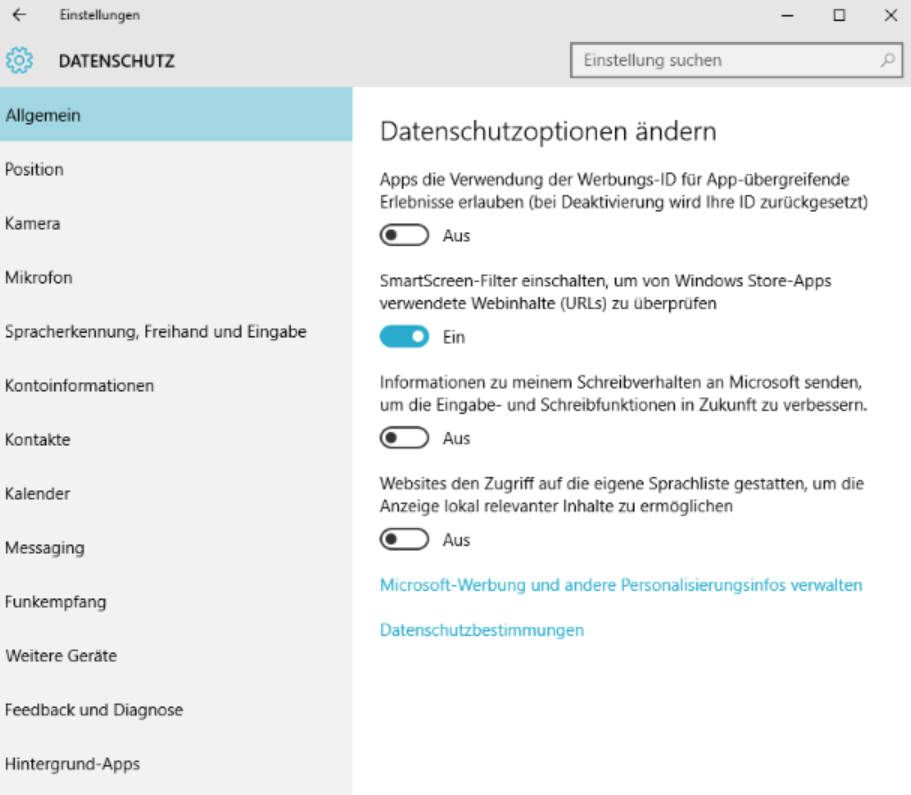
\includegraphics[width=0.7\textwidth]{img/windows10.png}
    \end{center}
\end{frame}

\note{Windows 10 ist ein gutes Beispiel für unerwünschte, aber nicht versteckte Funktionalität. Wenn man in die Datenschutzeinstellungen guckt, sieht man diverse sensitive Daten, die Windows - teils sogar voreingestellt aktiviert - an seine Server übertragen möchte. Darunter (auf dem Screenshot) befinden sich Punkte wie \"Schreibverhalten analysieren\". Das Schreibverhalten (wie man tippt, welche zeitlichen Abstände zwischen den Buchstaben) ist für jeden Menschen eindeutig und darüber kann man - einmal gespeichert - eine Person ohne weitere Kenntnisse an einem fremden PC wiedererkennen.}

\begin{frame}
  \frametitle{Unerwünschte Funktionalität}
  \begin{center}
    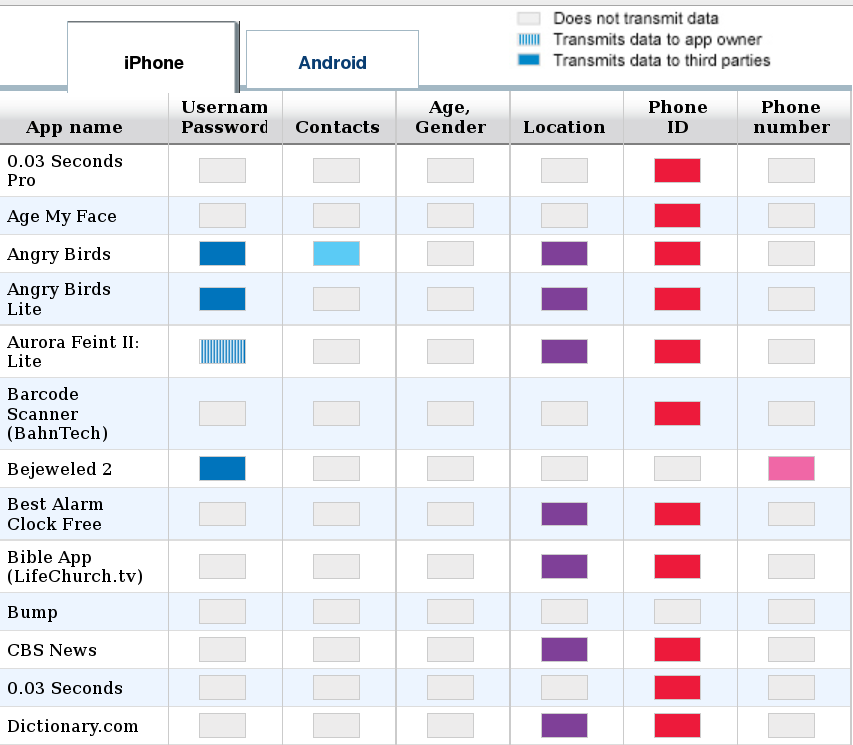
\includegraphics[width=7cm]{img/backdoor-apps.png}
  \par\end{center}
\end{frame}

\note{Apps haben häufig unerwünschte Nebenfunktionen, die dem Nutzer üblicherweise nicht ersichtlich sind. Es gibt lange Listen im Internet, die aufzeigen welche Apps welche Daten preisgeben und ob sie dies nur an die eigenen Server senden oder auch an Drittfirmen weitergeben. Auf dem Screenshot ist beispielsweise Angry Birds zu sehen, das eine große Reihe von Daten - unter anderem die eigene Identität, der Username, sein Passwort etc. auch an Dritte weitergibt.}
